\documentclass[UTF8,a4paper,10pt,fontset=fandol]{ctexart}
\usepackage[top=15mm,bottom=16mm,left=17mm,right=17mm]{geometry}
\usepackage{amsmath,amssymb,booktabs,graphicx,caption,hyperref,etoolbox,array,tabularx}
\usepackage{tikz}
\hypersetup{colorlinks=true,urlcolor=blue!50!black,linkcolor=black}
\captionsetup{font=small,skip=3pt,hypcap=false}
\ctexset{section={format=\large\bfseries,beforeskip=7pt,afterskip=4pt},
subsection={format=\normalsize\bfseries,beforeskip=5pt,afterskip=2pt}}
\setlength{\parskip}{3pt}
\setlength{\parindent}{2em}
\setlength{\tabcolsep}{5pt}
\linespread{1.05}
\newcommand{\fig}[3]{\begin{center}\includegraphics[width=#2\textwidth]{../results/figures/#1.pdf}\captionof{figure}{#3}\end{center}}
\newcommand{\RepoURL}{https://github.com/wszkxlllll/AI_Lab2}
\newcommand{\StudentName}{周可轩}
\newcommand{\StudentID}{10234700473}

\begin{document}
\pagestyle{plain}
\noindent 代码仓库：\ifdefempty{\RepoURL}{待填写实验二仓库地址}{\expandafter\url\expandafter{\RepoURL}}
\begin{center}
{\LARGE\bfseries 实验二：搜索算法}\par\vspace{4pt}
启发函数、剪枝顺序与有限深度决策\par
\vspace{3pt}姓名：\StudentName\qquad 学号：\StudentID
\end{center}

\section{实验目标与算法设计}
这次实验先完成四道题，再围绕三个问题继续探索：启发函数怎样减少寻路开销；访问顺序为什么影响剪枝；有限深度搜索能否通过更好的叶子评价改善首步选择。比较过程中同时记录答案、搜索量和时间，用具体路径与行动序列解释结果。

\begin{center}\small
\begin{tabular}{llll}
\toprule 题目 & 状态／目标 & 规则中的关键区别 & 规定样例结果\\\midrule
迷宫 & 当前格子／最短路径 & 四方向、每步代价 1 & 7 步、8 个坐标\\
加权地形 & 当前格子／最小代价 & 支付进入代价，E 免费 & 总代价 7\\
博弈树 & 当前节点与玩家／根节点值 & MAX 先手，从左到右 & 得分 5\\
宝藏分配 & 双方位置、宝藏与收益／首步 & A→B→A→B，特殊格代价 1 & H=2：T2，$-1$；H=4：T3，3\\
\bottomrule
\end{tabular}\end{center}

\subsection{A* 的状态、队列与最优性条件}
格子坐标为 $(r,c)$，维护起点到当前节点的已知最小代价 $g$、估计剩余代价 $h$ 和前驱。优先队列按 $f=g+h$ 取节点；找到更小的 $g$ 时更新前驱并重新入堆。旧堆项通过代价核对跳过，终点从队列取出时恢复路径。相同 $f$ 下分别比较先进先出（FIFO）、较大 $g$ 优先和较小 $g$ 优先。
\[
\text{可采纳性： }h(n)\le h^*(n),\qquad
\text{一致性： }h(n)\le c(n,n')+h(n'),\quad h(E)=0.
\]
一致性使路径上的 $f$ 不下降，节点以最小 $f$ 取出时，其最短到达代价已经确定。实现仍允许关闭节点被更小的 $g$ 重新打开，便于观察启发不一致时的行为。

\textbf{重开节点的小例子。}设置两条路线 $S\to A\to G$ 的边权为 $(3,3)$，$S\to B\to A\to G$ 为 $(1,1,3)$，取 $h(A)=0,h(B)=4,h(S)=h(G)=0$。各估计均为下界，但边 $B\to A$ 违反一致性。A* 先以 $g=3$ 关闭 A，随后从 B 找到 $g=2$。允许重开时得到最优代价 5，关闭后拒绝更新则得到 6；记录中发生了一次重开。

\subsection{Minimax 与 Alpha-beta}
叶子返回评价值，MAX 节点取子节点最大值，MIN 节点取最小值。Alpha-beta 维护 MAX 已有的下界 $\alpha$ 与 MIN 已有的上界 $\beta$：MAX 更新 $\alpha\leftarrow\max(\alpha,v)$，MIN 更新 $\beta\leftarrow\min(\beta,v)$，当 $\alpha\ge\beta$ 时停止搜索后续子分支。题目三使用完整树，题目四在宝藏取完或深度耗尽时评价。

\subsection{统一记录与核对}
为了比较搜索效率，记录寻路过程中展开的节点数、等待搜索的队列最大长度，以及博弈搜索访问的节点数和剪枝次数。寻路到达终点后停止展开，博弈访问数则包含根节点和叶子。每项实验先运行一次，再重复计时七次，取中位数。寻路计时包括地图处理、搜索和路径恢复；博弈计时包括行动排序和局面评价，宝藏之间的距离预先计算并单独计时。

为了检查结果是否正确，使用其他方法进行对照：随机小地图上的 A* 路径代价与 Floyd--Warshall 的结果比较，Alpha-beta 的回传值与完整 Minimax 比较，宝藏题则枚举完整行动序列核对最终收益。同时检查启发函数是否满足一致性。实验使用固定随机种子 66、88，并保存生成的地图，方便重复实验。

\newpage
\section{题目一、二：路径代价与启发函数}
\fig{given_paths}{0.80}{两题返回的路径。左图为 7 步；右图为 8 步，最后一步进入 E 免费。深色格为障碍，棕色格的进入代价较高。}

迷宫路径为 $(0,0)\to(0,1)\to(0,2)\to(1,2)\to(1,3)\to(1,4)\to(2,4)\to(3,4)$。加权题选择左侧与下方通道，避开代价 8 的地形，其逐步累计如下。
\begin{center}\small
\begin{tabular}{lrrrrrrrrr}
\toprule 坐标 & (0,0)&(1,0)&(2,0)&(3,0)&(3,1)&(3,2)&(4,2)&(4,3)&(4,4)\\\midrule
本步代价 &0&1&1&1&1&1&1&1&0\\
累计代价 &0&1&2&3&4&5&6&7&7\\\bottomrule
\end{tabular}\end{center}

\subsection{最后一步免费，怎样估计剩余代价}
曼哈顿距离 $D=|r-r_E|+|c-c_E|$ 是当前位置与终点的行差、列差之和，表示忽略障碍时最少还要走几步。题目一每步代价为 1，因此用 $h=D$。题目二最后一步进入 E 免费，其余格子最低代价为 1，因此改用 $h=\max(D-1,0)$。例如至少还要走 5 步，其中最后一步免费，剩余代价至少为 4；已经到达终点时取 0。

若换一张地图，普通格子的最低代价为 $m$，就用 $h=m\max(D-1,0)$。这里的 $m$ 从终点以外的可通行格子中取最小值，乘以它是把步数换成代价。步数和每步价格都取最低值，因此估计不会高于真实代价。走向普通格子时，估计最多减少 $m$，实际至少支付 $m$；走入免费终点时，两端估计均为 0。这也满足一致性要求：估计的下降量不超过本步实际代价。

为检查是否高估，先用 Dijkstra 算出每个格子到终点的真实最小代价，再与 $h$ 比较。原始曼哈顿距离在 20 个位置高估，修正后为 0；另逐条检查一致性，违反条件的边从 2 条降为 0。两种估计在给定样例上都找到总代价 7 的路径。

\begin{center}\small
\captionof{table}{搜索中实际检查邻居的格子数（扩展数），终点不计入。三种策略所得最优代价一致。}
\begin{tabular}{lrrrr}
\toprule 场景 & $h=0$／FIFO & 下界估计／FIFO & 下界估计／大 $g$ & 最优代价\\\midrule
题目一 & 15 & 13 & 7 & 7 \\
题目二 & 14 & 10 & 10 & 7 \\
空图 80×80 & 6399 & 6399 & 158 & 158 \\
障碍 80×80（66） & 4751 & 2158 & 485 & 158 \\
地形 80×80（88） & 5418 & 3448 & 3324 & 204 \\
不可达 20×20 & 200 & 200 & 200 & 无路
\\\bottomrule
\end{tabular}\end{center}

\subsection{分数相同时，先检查哪个位置}
表中 $h=0$ 表示只按已走代价搜索；下界估计采用前述方法。所有策略先选 $f=g+h$ 最小的节点。同分时，FIFO 选择先加入队列的节点；大 $g$ 优先选择已走代价较大的节点。

80×80 空地图从左上角到右下角至少要走 $79+79=158$ 步。沿最短路线每前进一步，$g$ 增加 1、$h$ 减少 1，总分 $f$ 始终为 158。因此许多位置同分：FIFO 逐层向外搜索，检查了终点以外的 6,399 个格子；大 $g$ 优先沿一条最短路线继续推进，只检查了 158 个格子。两者找到的路线同样长。

终点被整行障碍隔开时，三种策略都检查了起点一侧全部 200 个可达格子，才确认无路。大 $g$ 优先累计向队列加入 352 条记录，其中 152 条因后来找到更短路线而过期。更新时新记录入队，旧记录等取出时再跳过，所以同一格子可能同时占用多条记录。队列最大长度由 FIFO 的 11 增至 153，增加了空间开销。表中的加权地图则只有较小变化：展开数从 3448 降到 3324；同分规则只在 $f$ 相等时影响选择。

\newpage
\section{题目三：数值回传、界与访问顺序}
\fig{tree_pruning}{0.86}{按给定输入展开的博弈树。根节点值为 5；橙色分支在从左到右搜索时被剪去。返回的 $\ge6$ 表示当前已知下界。}

先计算左下分支，MAX 从 3、5 中取 5，左侧 MIN 的 $\beta$ 随之变为 5。接着访问其右侧 MAX，读到叶子 6 后已有 $\alpha=6\ge\beta=5$，于是跳过叶子 9。左侧 MIN 仍选择 5。右侧 MIN 从 9、2 中取 2，根节点最终取 $\max(5,2)=5$。

\textbf{剪枝返回的是足够决策的信息。}被截断的 MAX 分支返回 6，已知真实值至少为 6；完整展开的精确值是 9。父节点拿它与已有的 5 比较，已足以确定选择。实现会在跟踪记录中标出上界、下界和精确值。给定构造代码复用了 $(6,9)$ 节点，输入 JSON 中它出现两次，本实验按两次到达分别计数，因此完整搜索访问 15 个节点、评价 8 个叶子位置。

\begin{center}\small
\captionof{table}{给定树的访问顺序对照，所有方法根节点值均为 5。}
\begin{tabular}{llrrrr}
\toprule 方法 & 顺序 & 访问节点 & 叶子评价 & 剪枝事件 & 时间/ms\\\midrule
Minimax & 从左到右 & 15 & 8 & 0 & 0.022 \\
Alpha-beta & 从左到右 & 14 & 7 & 1 & 0.023 \\
Alpha-beta & 反向 & 14 & 7 & 1 & 0.023 \\
Alpha-beta & 随机（66） & 11 & 5 & 2 & 0.072
\\\bottomrule
\end{tabular}\end{center}

\subsection{把同一组分数换一种访问顺序}
为了观察规模变化，进一步生成分支数 2、3、4，深度 4--8 的 12 棵树，叶子分数在 $[-20,20]$ 中取整数。原顺序、反顺序和随机顺序使用相同树；随机排列由种子与节点名决定，保证某处分支被剪掉后，其他节点的排列保持一致。
\fig{tree_order}{0.86}{两棵三叉、深度 6 的树。Minimax 均访问 1,093 个节点，Alpha-beta 的访问量随顺序变化；两种子对应的根值分别为 $-7$、$-5$。}

种子 66 的树中，原顺序比反顺序更省节点；种子 88 的树中，反顺序更省。原因在于有用的界出现时间不同：MAX 较早找到高值、MIN 较早找到低值时，更容易截断剩余分支。

以种子 66 的三叉深度 6 树为例，随机顺序的 Alpha-beta 访问 474 个节点，少于原顺序 Minimax 的 1093 个；耗时却为 2.650 ms，高于后者的 1.819 ms。节点减少与运行加速需要分别观察。



\newpage
\section{题目四：宝藏分配与搜索深度}
\begin{center}
\begin{minipage}[c]{.25\textwidth}\centering
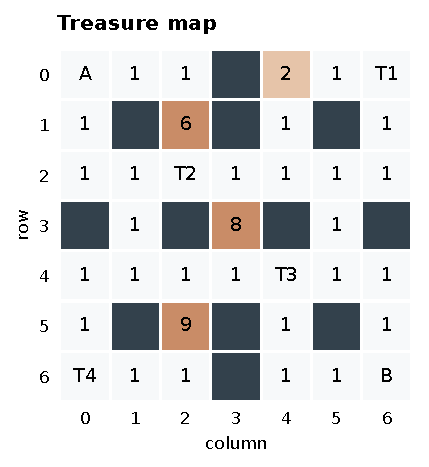
\includegraphics[width=\linewidth]{../results/figures/treasure_map.pdf}
\end{minipage}\hfill
\begin{minipage}[c]{.58\textwidth}\centering\small
\begin{tabular}{lrrrrrr}
\toprule & A&B&T1&T2&T3&T4\\\midrule
A & 0 & 12 & 10 & 4 & 8 & 8 \\
B & 12 & 0 & 8 & 8 & 4 & 10 \\
T1 & 10 & 8 & 0 & 6 & 6 & 12 \\
T2 & 4 & 8 & 6 & 0 & 6 & 6 \\
T3 & 8 & 4 & 6 & 6 & 0 & 6 \\
T4 & 8 & 10 & 12 & 6 & 6 & 0
\\\bottomrule
\end{tabular}\par\vspace{7pt}
宝藏价值：T1=9，T2=6，T3=7，T4=7。\par
A、B 和宝藏格进入代价均为 1。
\end{minipage}
\captionof{figure}{题目四地图及 A* 算出的距离矩阵，名称顺序固定为 A、B、T1、T2、T3、T4。}
\end{center}

\subsection{先用 A* 算出移动代价}
对 A、B、T1--T4 中每一对不同位置运行 A*，共计算 $6\times5=30$ 次。每次把目的位置作为终点，$g$ 累加沿途进入格子的代价，启发函数取曼哈顿距离 $h=|r-r_{\text{目标}}|+|c-c_{\text{目标}}|$。本题每步至少花费 1，进入宝藏格也要支付 1，因此直接用最少步数估计剩余代价，无需像题目二那样减去最后一步。每移动一步，$h$ 最多减少 1，而实际代价至少为 1，所以满足一致性。

表中的“距离”是最小移动代价，例如 A 到 T2 为 4，后续博弈直接查表。对角线为 0；各标记格进入代价相同，路线反向经过时总代价相同，因此表格对称。

\subsection{把轮流取宝藏展开成树}
树中每条边表示当前玩家选取一个宝藏，每个节点记录双方位置、剩余宝藏和双方累计收益。取到宝藏后，行动玩家移动到该处，并获得“宝藏价值减去移动代价”的收益；只删除选定宝藏，路过其他宝藏不收取，双方也不挡路。统一用 $U=s_A-s_B$ 评价：A 希望它越大越好，取最大值；B 希望它越小越好，取最小值。

\begin{center}
\begin{tikzpicture}[x=1cm,y=1cm,every node/.style={font=\small,align=center},choice/.style={draw,rounded corners=2pt,minimum width=8mm,inner sep=2pt},every path/.style={draw=black!55}]
\node (root) at (0,0) {开始};
\node at (2,1.4) {第 1 步：A\\4 种选择};
\node at (5,1.4) {第 2 步：B\\3 种选择};
\node at (8,1.4) {第 3 步：A\\2 种选择};
\node at (11,1.4) {第 4 步：B\\1 种选择};
\node[choice] (a1) at (2,.8) {T1};
\node[choice] (a2) at (2,.25) {T2};
\node[choice] (a3) at (2,-.3) {T3};
\node[choice] (a4) at (2,-.85) {T4};
\foreach \n in {a1,a2,a3,a4} \draw[->] (root.east)--(\n.west);
\node[choice] (b1) at (5,.8) {T1};
\node[choice] (b3) at (5,.1) {T3};
\node[choice] (b4) at (5,-.6) {T4};
\foreach \n in {b1,b3,b4} \draw[->] (a2.east)--(\n.west);
\node[choice] (c1) at (8,.5) {T1};
\node[choice] (c4) at (8,-.3) {T4};
\draw[->] (b3.east)--(c1.west); \draw[->] (b3.east)--(c4.west);
\node[choice] (d4) at (11,.5) {T4};
\node[choice] (d1) at (11,-.3) {T1};
\draw[->] (c1.east)--(d4.west); \draw[->] (c4.east)--(d1.west);
\node at (5,-1.15) {$H=2$ 停在此列};
\node at (11,-1.15) {$H=4$ 停在此列};
\end{tikzpicture}
\captionof{figure}{从左向右展开选择树，方框标出本次取走的宝藏。以 T2→T3 为例展示后续分支，其余省略。}
\end{center}

$H=2$ 只看 A、B 各行动一次后的收益差；$H=4$ 看完四次行动。评价从右向左回传：B 的选择取最小值，A 的选择取最大值，最终确定第一步。

\begin{center}\small
\begin{minipage}[t]{.39\textwidth}\centering
\captionof{table}{各首步的回传值。}
\begin{tabular}{lrrrr}
\toprule 首步&T1&T2&T3&T4\\\midrule
$H=2$&$-4$&$-1$&$-2$&$-4$\\
$H=4$&$-5$&1&3&$-7$\\\bottomrule
\end{tabular}
\end{minipage}\hfill
\begin{minipage}[t]{.59\textwidth}\centering
\captionof{table}{完整搜索的一条最优行动序列。}
\setlength{\tabcolsep}{3pt}
\begin{tabular}{clrrcr}
\toprule 玩家&移动&代价&收益&$(s_A,s_B)$&$U$\\\midrule
A&A→T3&8&$-1$&$(-1,0)$&$-1$\\
B&B→T1&8&1&$(-1,1)$&$-2$\\
A&T3→T2&6&0&$(-1,1)$&$-2$\\
B&T1→T4&12&$-5$&$(-1,-4)$&3\\\bottomrule
\end{tabular}
\end{minipage}
\end{center}

浅层搜索选择 T2，看到 A 先得 2、B 取 T3 得 3，当前差值为 $-1$。把 T2 首步固定后继续搜索到终局，结果为 1；完整搜索选择 T3，终局为 3，所以本例浅层首步损失为 2。

完整搜索中，A 累计 $-1$，B 累计 $-4$，最终 $U=-1-(-4)=3$。后两次行动使完整搜索改变了首步选择。

\begin{center}\small
\captionof{table}{综合题的节点开销。收益顺序按当前玩家即时收益从高到低排列。}
\begin{tabular}{crrrr}
\toprule 深度 & Minimax & AB 原顺序 & AB 反顺序 & AB 收益顺序\\\midrule
2&17&13&16&11\\
4&65&47&46&37\\\bottomrule
\end{tabular}\end{center}
距离矩阵预计算中位耗时 1.607 ms。深度 4 的 Alpha-beta 从原顺序到收益顺序，访问量由 47 降至 37，决策时间分别为 0.112、0.115 ms。计时包含收益排序与状态更新，所有顺序均保持根值 3。


\newpage
\section{拓展：用剩余机会改善浅层评价}
在 $H=2$ 截止时还剩两个宝藏，只看当前收益会遗漏下一次移动的影响。这里尝试增加双方最佳剩余即时收益之差，权重在实验前固定为 1：
\[
\widehat V(s)=U(s)+\max_{i\in R}\{V_i-d(p_A,T_i)\}
                     -\max_{i\in R}\{V_i-d(p_B,T_i)\}.
\]
宝藏取完时直接返回 $U$。公式允许负收益，因为规则要求每回合选取宝藏。实现仅在深度耗尽的叶子计算这项估计，搜索仍为两层；距离均由预计算矩阵提供。

\subsection{用同一终局标准评价首步}
按种子 66、88 各取前 10 张连通地图，共尝试 24 张，4 张因标记不连通被筛除。地图为 7×7，障碍概率 0.12，普通地形从 $[1,1,1,2,5]$ 抽取，四个宝藏价值在 $[6,14]$ 中取整数。保存全部接受输入及筛选记录，比较贪心、原始两层、机会评价两层和完整四层搜索。

每种方法先选第一步，再固定该行动，用完整 Minimax 算出双方后续最优应对下的终局收益差 $U(a)$。首步损失 $R=U^*-U(a)$ 表示比最优终局少了多少：例如最优为 11，选定首步后只能达到 3，损失就是 8；损失为 0 表示选中了最优首步。计时只包含当前方法选择首步的过程，终局核验另算。

\begin{center}\small
\captionof{table}{20 张自设地图的决策质量。时间为各场景决策时间中位数的中位数。}
\begin{tabular}{lrrrr}
\toprule 方法 & 最优首步命中 & 平均损失 & 最大损失 & 时间/ms\\\midrule
即时收益贪心 & 11/20 & 3.20 & 14 & 0.0018 \\
H=2，当前收益 & 15/20 & 1.25 & 8 & 0.0622 \\
H=2，机会评价 & 17/20 & 0.30 & 3 & 0.0842 \\
H=4，完整搜索 & 20/20 & 0.00 & 0 & 0.2041
\\\bottomrule
\end{tabular}\end{center}
\fig{decision_quality}{0.90}{左图每组对应同样的 20 张地图，点越低，首步选择越好；零损失点可能重合。右图显示加入机会评价后，5 张改善、12 张损失相同、3 张变差。}

\subsection{改善与失败的具体原因}
\begin{center}\small
\captionof{table}{两个案例中的候选首步。估计分数用于选首步，真实终局由固定首步后的完整搜索计算。}
\begin{tabular}{llrrr}
\toprule 场景 & 首步 & 原始两层估计 & 机会两层估计 & 真实终局收益差\\\midrule
66--7&T2&$-1$&$-7$&3\\
66--7&T3&$-2$&3&11\\
88--2&T2&$-9$&$-6$&$-5$\\
88--2&T3&$-8$&$-6$&$-2$\\\bottomrule
\end{tabular}\end{center}

场景 66--7 中，原始评价选 T2，机会评价改选 T3，真实终局从 3 提高到 11。T3 对应的最优行动序列中，B 最后从 T4 到 T1 要付出 22 的移动代价，拉低了 B 的收益。两层搜索尚未展开这一步，加入剩余机会后，这次选中了终局更好的首步。

场景 88--2 中，原始评价选择 T3；机会评价把 T2、T3 都算成 $-6$，按固定顺序先选 T2。真实终局却从 $-2$ 降到 $-5$，损失增加 3：有优劣的两个选择被估成了一样好。课程给定地图上，两种评价都选 T2，最终收益差均为 1。

\subsection{总结与后续方向}
同分排序在空地图上明显减少扩展，遇到不可达目标时则增加堆空间开销。Alpha-beta 的正确性来自上下界，效率取决于界出现的先后和排序成本。机会评价在 20 张地图上改善 5 次、变差 3 次、持平 12 次，平均首步损失从 1.25 降到 0.30；进一步改进可把双方对同一宝藏的争夺和先手信息纳入估计。

\end{document}
